\documentclass{report}
\usepackage{yfonts}
\usepackage{fontspec}
\usepackage[english]{babel}
\usepackage{pgfplots}
\pgfplotsset{width=10cm,compat=1.17}
\usepackage{xcolor}
\definecolor{powderBlue}{HTML}{B0E0E6}
\definecolor{forestGreen}{HTML}{014421}
\usepackage{amsmath}
\usepackage{amssymb}
\title{New Resist \& Damage}
\author{Scot MoonShade\\
\texttt{@\textfrak{ShadowScott}\#1234}
\and
Nate ShadowBringer\\
\texttt{@PhantomNate\#0001}
\and
Juan FireCaster\\
\texttt{@jjeastside\#7289}
\and
Wolf Stalker \\
\texttt{@Lucyfer\#5969}
\and
Daniel FrostHeart \\
\texttt{@Mayonnaisinator\#9263}
}
\date{16 April 2021}
\begin{document}
    \maketitle
    \section*{Damage}
    \subsection*{PvP}
    \subsubsection{Raw}
    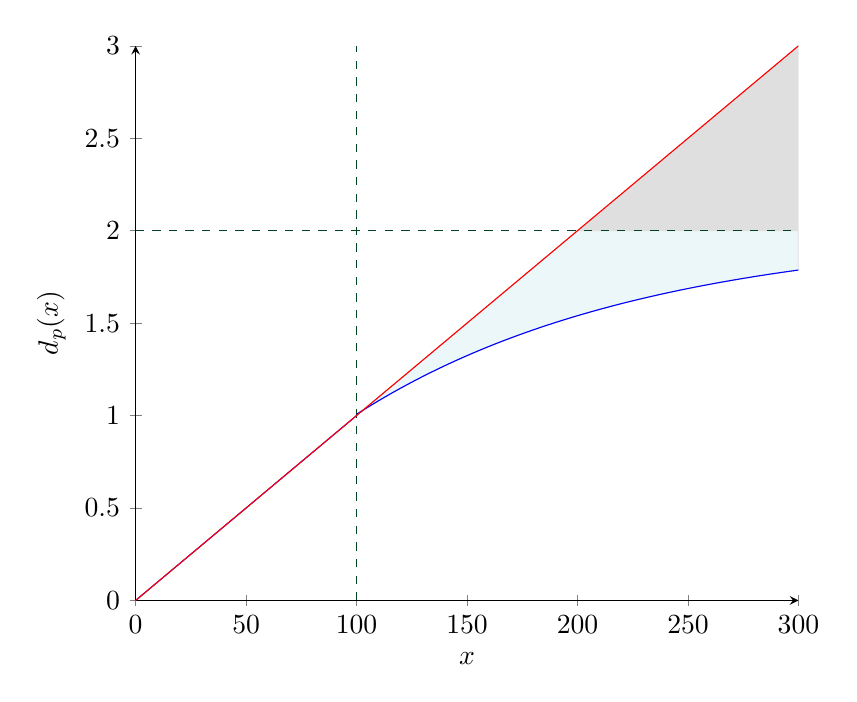
\begin{tikzpicture}
        \begin{axis}[
            axis lines = left,
            legend pos = south west,
            xlabel = $x$,
            ylabel = {$d_{p}(x)$},
        ]
        \draw[fill=gray!25,draw=gray!25] plot[smooth,samples=100,domain=100:300] (\x,{\x/100}) -- 
        plot[smooth,samples=100,domain=300:100] (\x,{2-(2/(e^(0.00770163*\x-0.0701635)))});
        \draw[fill=powderBlue!25,draw=gray!25] plot[smooth,samples=100,domain=100:200] (\x,{\x/100}) -- 
        plot[smooth,samples=100,domain=200:300] (\x,{2}) -- 
        plot[smooth,samples=100,domain=300:100] (\x,{2-(2/(e^(0.00770163*\x-0.0701635)))});
        \draw[dashed, draw = forestGreen](0,2)--(300,2);
        \draw[dashed, draw = forestGreen](100,0)--(100,3);
        \addplot [
            domain=0:100, 
            samples=100, 
            color=blue,
        ]
        {x/100};
        \addplot [
            domain=100:300, 
            samples=250, 
            color=blue,
            ]
        {2-(2/(e^(0.00770163*x-0.0701635)))};
        \addplot[
            domain=0:300,
            samples=50,
            color=red,
        ]
        {x/100};
        \end{axis}
    \end{tikzpicture}
    \begin{center}
        \begin{equation*}
            d_{p}(x) = 
            \begin{cases}
                x; 0 \le x \le 100 \\
                \ \\
                2-\dfrac{2}{e^{a_1x-b_1}}; 100 < x
            \end{cases}
        \end{equation*}
    \end{center}
    \subsubsection*{Rate of Change ($\Delta$)}
    \begin{tikzpicture}
        \begin{axis}[
            axis lines = left,
            legend pos = south west,
            ylabel = ${d_p}^{\prime}(x)$,
            xlabel = $x$,
            ymax = 0.0105
        ]
        \draw[dashed, color = forestGreen](100,0)--(100,0.0105);
        \addplot[
            domain = 0:100,
            samples = 5,
            color = blue
        ]
        {1/100};
        \addplot[
            domain = 100:300,
            samples = 300,
            color = blue
        ]
        {0.01540326*e^(-0.00770163*x+0.0701635)};
        \filldraw[black](100,0.01) circle (2pt);
        \draw[color = black, fill = white](100,0.00764903) circle (2pt);
        \end{axis}
    \end{tikzpicture}
    \begin{equation*}
        {d_p}^{\prime}(x) = 
        \begin{cases}
            0.01; 0 \le x \le 100 \\
            \ \\
            \alpha_{1} \cdot e^{\beta_1x+\gamma_1}; 100 < x
        \end{cases}
    \end{equation*}
    \newpage{}
    \subsection*{PvE}
    \subsubsection*{Raw}
    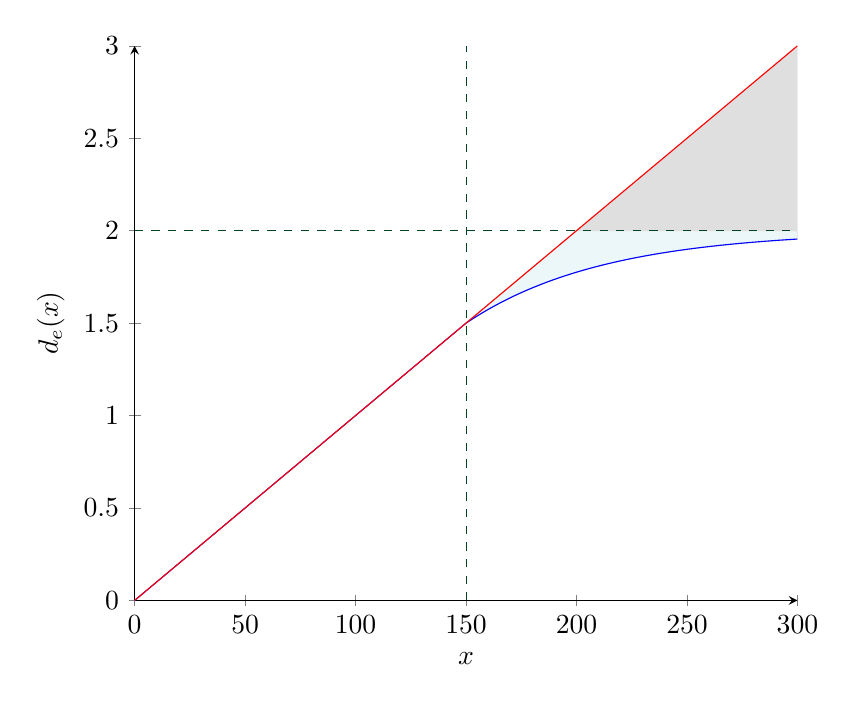
\begin{tikzpicture}
        \begin{axis} [
            axis lines = left,
            legend pos = south west,
            xlabel = $x$,
            ylabel = $d_{e} (x)$,
        ]
        \draw[fill=gray!25,draw=gray!25] plot[smooth,samples=100,domain=150:300] (\x,{\x/100}) -- 
        plot[smooth,samples=100,domain=300:150] (\x,{2-(2/(e^(0.0160168*\x-1.01623692)))});
        \draw[fill=powderBlue!25,draw=gray!25] plot[smooth,samples=100,domain=150:200] (\x,{\x/100}) -- 
        plot[smooth,samples=100,domain=200:300] (\x,{2}) -- 
        plot[smooth,samples=100,domain=300:150] (\x,{2-(2/(e^(0.0160168*\x-1.01623692)))});
        \draw[dashed, draw = forestGreen](0,2)--(300,2);
        \draw[dashed, draw = forestGreen](150,0)--(150,3);
        \addplot[
            domain = 0:150,
            samples = 50,
            color = blue,
        ]
        {x/100};
        \addplot [
            domain = 150:300,
            samples = 250,
            color = blue,
        ]
        {2-(2/(e^(0.0160168*x-1.01623692)))};
        \addplot[
            domain = 0:300,
            samples = 50,
            color = red,
        ]
        {x/100};
        \end{axis}
    \end{tikzpicture}
    \begin{center}
        \begin{equation*}
            {d_{e}}(x) = 
            \begin{cases}
                x; 0 \le x \le 150 \\
                \ \\
                2-\dfrac{2}{e^{a_2x-b_2}}; 150 < x
            \end{cases}
        \end{equation*}
    \end{center}
    \subsubsection*{Rate of Change ($\Delta$)}
    \begin{tikzpicture}
        \begin{axis}[
            axis lines = left,
            legend pos = south west,
            ylabel = ${d_e}^{\prime}(x)$,
            xlabel = $x$,
            ymax = 0.0105
        ]
        \draw[dashed, color = forestGreen](150,0)--(150,0.0105);
        \addplot[
            domain = 0:150,
            samples = 5,
            color = blue
        ]
        {1/100};
        \addplot[
            domain = 150:300,
            samples = 300,
            color = blue
        ]
        {0.0320336*e^(-0.0160168*x+1.01623692)};
        \filldraw[black](150,0.01) circle (2pt);
        \draw[color = black, fill = white](150,0.00800849) circle (2pt);
        \end{axis}
    \end{tikzpicture}
    \begin{equation*}
        {d_e}^{\prime}(x) = 
        \begin{cases}
            0.01; 0 \le x \le 150 \\
            \ \\
            \alpha_{2} \cdot e^{\beta_2x+\gamma_2}; 150 < x
        \end{cases}
    \end{equation*}
    \newpage{}
    \section*{Resist}
    \subsection*{PvP}
    \subsubsection{Raw}
    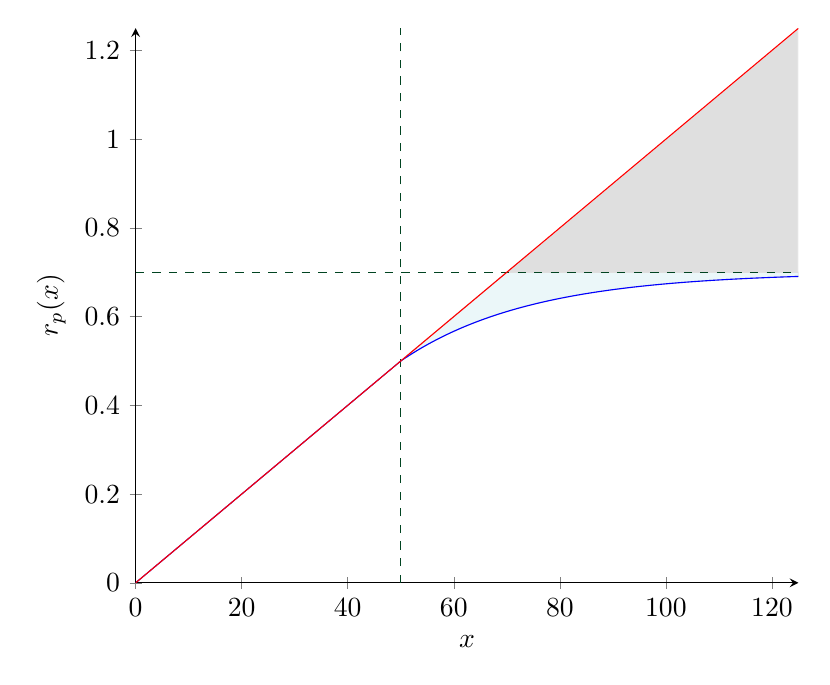
\begin{tikzpicture}
        \begin{axis}[
            axis lines = left,
            legend pos = south west,
            xlabel = $x$,
            ylabel = ${r_{p}}(x)$,
        ]
        \draw[fill=gray!25,draw=white!0] plot[smooth,samples=100,domain=50:125] (\x,{\x/100}) -- 
        plot[smooth,samples=100,domain=125:50] (\x,{0.7-((0.7)/(e^(0.04072764*\x-0.78361903))});
        \draw[fill=powderBlue!25,draw=gray!25] plot[smooth,samples=100,domain=50:75] (\x,{\x/100}) -- 
        plot[smooth,samples=100,domain=70:125] (\x,{0.7}) -- 
        plot[smooth,samples=100,domain=125:50] (\x,{0.7-((0.7)/(e^(0.04072764*\x-0.78361903))});
        \draw[dashed, draw = forestGreen](0,0.7)--(125,0.7);
        \draw[dashed, draw = forestGreen](50,0)--(50,1.25);
        \addplot[
            domain = 0:50,
            samples = 50,
            color = blue,
        ]
        {x/100};
        \addplot[
            domain = 50:125,
            samples = 150,
            color = blue,
        ]
        {0.7-((0.7)/(e^(0.04072764*x-0.78361903))};
        \addplot[
            domain = 0:125,
            samples = 50,
            color = red,
        ]
        {x/100};
        \end{axis}
    \end{tikzpicture}
    \begin{center}
        \begin{equation*}
            {r_{p}}(x) = 
            \begin{cases}
                x; 0 \le x \le 50 \\
                \ \\
                0.7-\dfrac{0.7}{e^{a_3x-b_3}}; 50 < x
            \end{cases}
        \end{equation*}
    \end{center}
    \subsubsection*{Rate of Change ($\Delta$)}
    \begin{tikzpicture}
        \begin{axis}[
            axis lines = left,
            legend pos = south west,
            ylabel = ${r_p}^{\prime}(x)$,
            xlabel = $x$,
            ymax = 0.0105
        ]
        \draw[dashed, color = forestGreen](50,0)--(50,0.0105);
        \draw[dashed, color = forestGreen](50,0.01)--(120,0.01);
        \addplot[
            domain = 0:50,
            samples = 5,
            color = blue
        ]
        {1/100};
        \addplot[
            domain = 50:125,
            samples = 300,
            color = blue
        ]
        {0.02850934*e^(-0.04072764*x+0.78361903)};
        \filldraw[black](50,0.01) circle (2pt);
        \draw[color = black, fill = white](50,0.00814552) circle (2pt);
        \end{axis}
    \end{tikzpicture}
    \begin{equation*}
        {r_p}^{\prime}(x) = 
        \begin{cases}
            0.01; 0 \le x \le 50 \\
            \ \\
            \alpha_{3} \cdot e^{\beta_3x+\gamma_3}; 50 < x
        \end{cases}
    \end{equation*}
    \newpage{}
    \section*{Definition of constants}
    \begin{tabular}{||c | c||}
        \hline
        \textbf{constant} & \textbf{value} \\
        \hline\hline
        $a_1$ & $0.00770162$ \\
        \hline
        $b_1$ & $0.0701635$ \\
        \hline
        $\alpha_1$ & $0.01540326$ \\
        \hline
        $\beta_1$ & $-0.00770163$ \\
        \hline
        $\gamma_1$ & $0.0701635$ \\
        \hline\hline
        $a_2$ & $0.0160168$ \\
        \hline
        $b_2$ & $-1.01623692$ \\
        \hline
        $\alpha_2$ & $0.0320336$ \\
        \hline
        $\beta_2$ & $-0.0160168$ \\
        \hline
        $\gamma_2$ & $1.01623692$ \\
        \hline\hline
        $a_3$ & $0.04072764$ \\
        \hline
        $b_3$ & $-0.7836190$ \\
        \hline
        $\alpha_3$ & $0.02850934$ \\
        \hline
        $\beta_3$ & $-0.04072764$ \\
        \hline
        $\gamma_3$ & $0.78361903$ \\
        \hline
    \end{tabular}
    \section*{Limit Definitions}
    The functions follow the following trends, with \textbf{\textit{absolute}} limits.
    \begin{align*}
        \lim_{x \to \infty} d(x) &= 2 \\
        \lim_{x \to \infty} {r_{p}}(x) &= 0.7
    \end{align*}
\end{document}